\section{The ATLAS Detector}%
\label{sec:atlas}

The ATLAS detector~\cite{PERF-2007-01}, shown in
\Cref{fig:atlas_detector_overview}, is a cylindrical particle detector
surrounding the LHC beamline at one of the IPs. The detector covers most of the
solid angle surrounding the IP to ensure that a large fraction of particles
produced in hard scattering reactions pass through the active detector volume.
% all detectable particles from collisions can be observed.
The central part of the ATLAS detector is referred to as the \emph{barrel},
while the two sections covering the solid angle close to the LHC beamline are
referred to as the \emph{end-caps}. Different layers of detector technologies
are concentrically arranged around the IP that, in conjunction, allow to detect
and identify different types of particles, enabling an almost full
interpretation of collision events.

\begin{figure}[htbp]
  \centering

  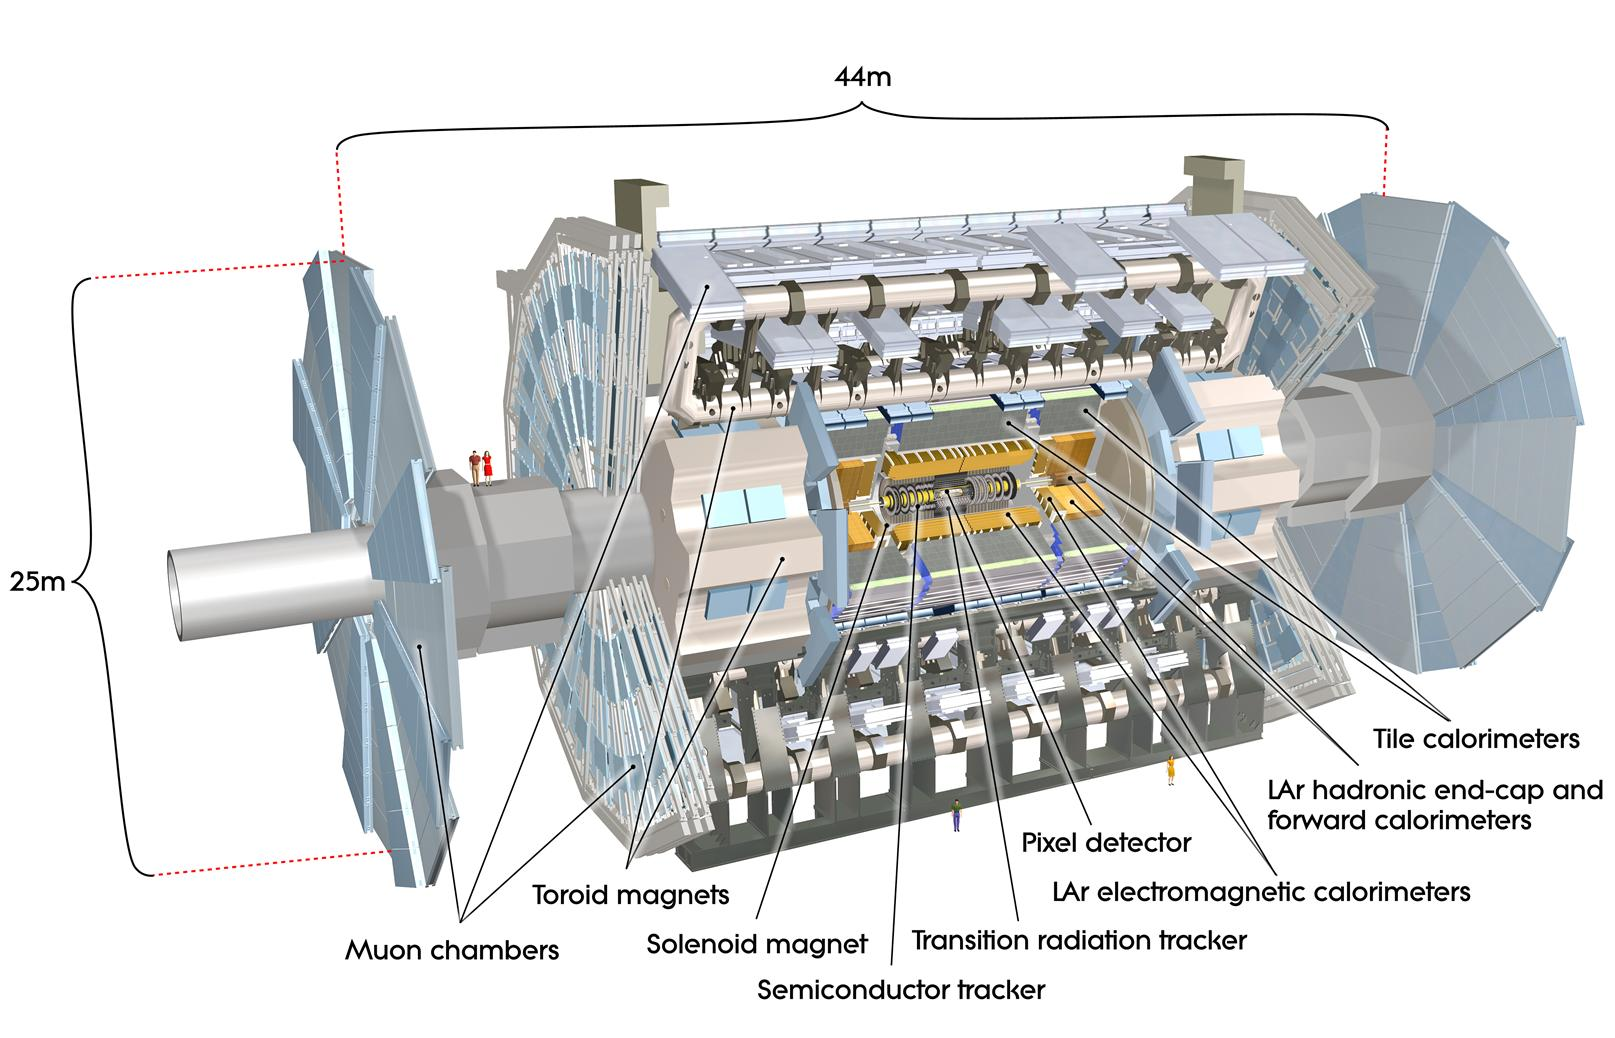
\includegraphics[width=0.76\textwidth]{atlas/atlas_overview}

  \caption[Overview of the ATLAS detector.]{Overview of the ATLAS detector. The
    image is taken from Ref.~\cite{PERF-2007-01}.}%
  \label{fig:atlas_detector_overview}
\end{figure}

The ATLAS experiment uses a right-handed Cartesian coordinate system with the
origin being located in the centre of the detector at the nominal IP. The axes
of the coordinate system are given as follows: the $x$-axis points to the centre
of the LHC, the $y$-axis points upwards, and the $z$-axis points along the LHC
beamline. The plane spanned by the $x$- and $y$-axes is referred to as the
transverse plane. A spherical coordinate system is used to specify directions in
three-dimensional space. The azimuthal angle, $\phi$, of this coordinate system
is defined as the angle in the transverse plane measured with respect to the
$x$-axis, and the polar angle, $\theta$, being the angle with respect to the
$z$-axis. With these coordinate systems, transverse momenta and energies are
defined as $\pT = \sqrt{p_x^2 + p_y^2} = p \sin\theta$ and $\ET = E \sin\theta$,
respectively. At hadron colliders, the polar angle is frequently given in terms
of the pseudorapidity $\eta$, which is defined as
\begin{align*}
  \eta = - \ln\tan\left( \frac{\theta}{2} \right) \,\text{.}
\end{align*}
Similarly, the angular separation between two particles is defined as
\begin{align*}
  \Delta R = \sqrt{\Delta \eta^2 + \Delta \phi^2} \,\text{,}
\end{align*}
where $\Delta \eta$ is the difference in pseudorapidity and $\Delta \phi$ the
smallest azimuthal separation between the particle momenta.

The main components of the ATLAS detector, going from the IP outwards, are the
\emph{Inner Detector} (ID) used for measuring the trajectories of charged
particles, the \emph{Calorimeters} used to destructively measure the energy of
most charged and neutral particles, and the \emph{Muon Spectrometer} (MS) used
to measure the trajectories of muons that can pass the calorimeters. Particles
in the ID are bent in the transverse plane due to a magnetic field of
\SI{2}{\tesla} field strength pointing along the $z$-axis that is produced by a
superconducting solenoid surrounding the ID.  The MS is equipped with
superconducting toroid magnets that bend the trajectories of muons in the
direction described by the $\eta$-coordinate. The curvature of charged-particle
trajectories in the ID and MS allows to determine the sign of the electric
charge and momentum of particles. The following sections summarise the
sub-systems of the ATLAS detector.


\subsection{The Inner Detector}

The ID, schematically depicted in \Cref{fig:atlas_inner_detector}, is the
innermost part of the ATLAS detector. It performs non-destructive measurements
of the trajectories of charged particles within $|\eta| < 2.5$ by measuring the
points where charged particles cross active detector layers. The measurement of
several points on the trajectory, and the known magnetic field in the ID, allows
to reconstruct the trajectory of the particle. The reconstructed trajectory is
referred to as the \emph{charged-particle track} and often abbreviated as
\emph{track}. The precise measurement of charged-particle tracks is important to
reconstruct the primary vertex (PV) of the hard interaction with high spatial
resolution, allowing to remove tracks from pile-up which are typically displaced
from the PV along the $z$-axis. Moreover, the accurate reconstruction of
secondary vertices, i.e.\ displaced vertices originating from decays of unstable
particles produced in the hard interaction, is crucial to identify jets
originating from $b$-quarks.% which hinges on the precision of the track
% reconstruction in the ID.

\begin{figure}[htbp]

  \begin{subfigure}[b]{0.55\textwidth}
    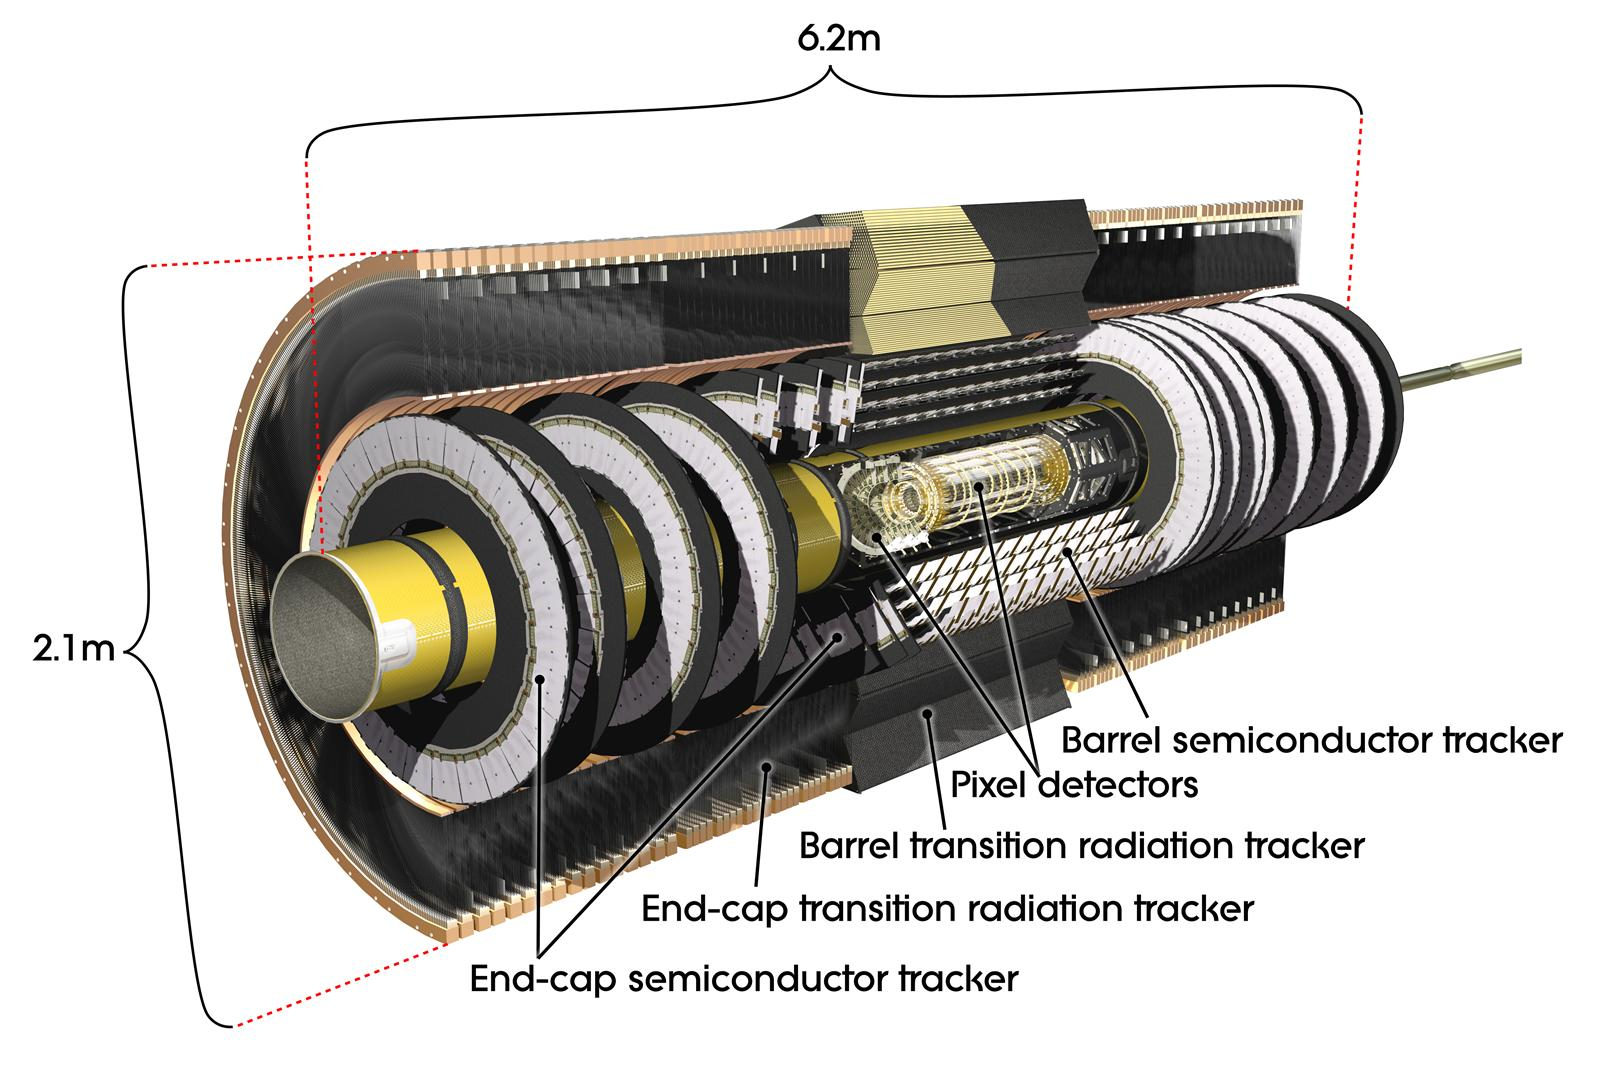
\includegraphics[width=\textwidth]{atlas/atlas_indet_1}%
    \subcaption{}
  \end{subfigure}\hfill%
  \begin{subfigure}[b]{0.45\textwidth}
    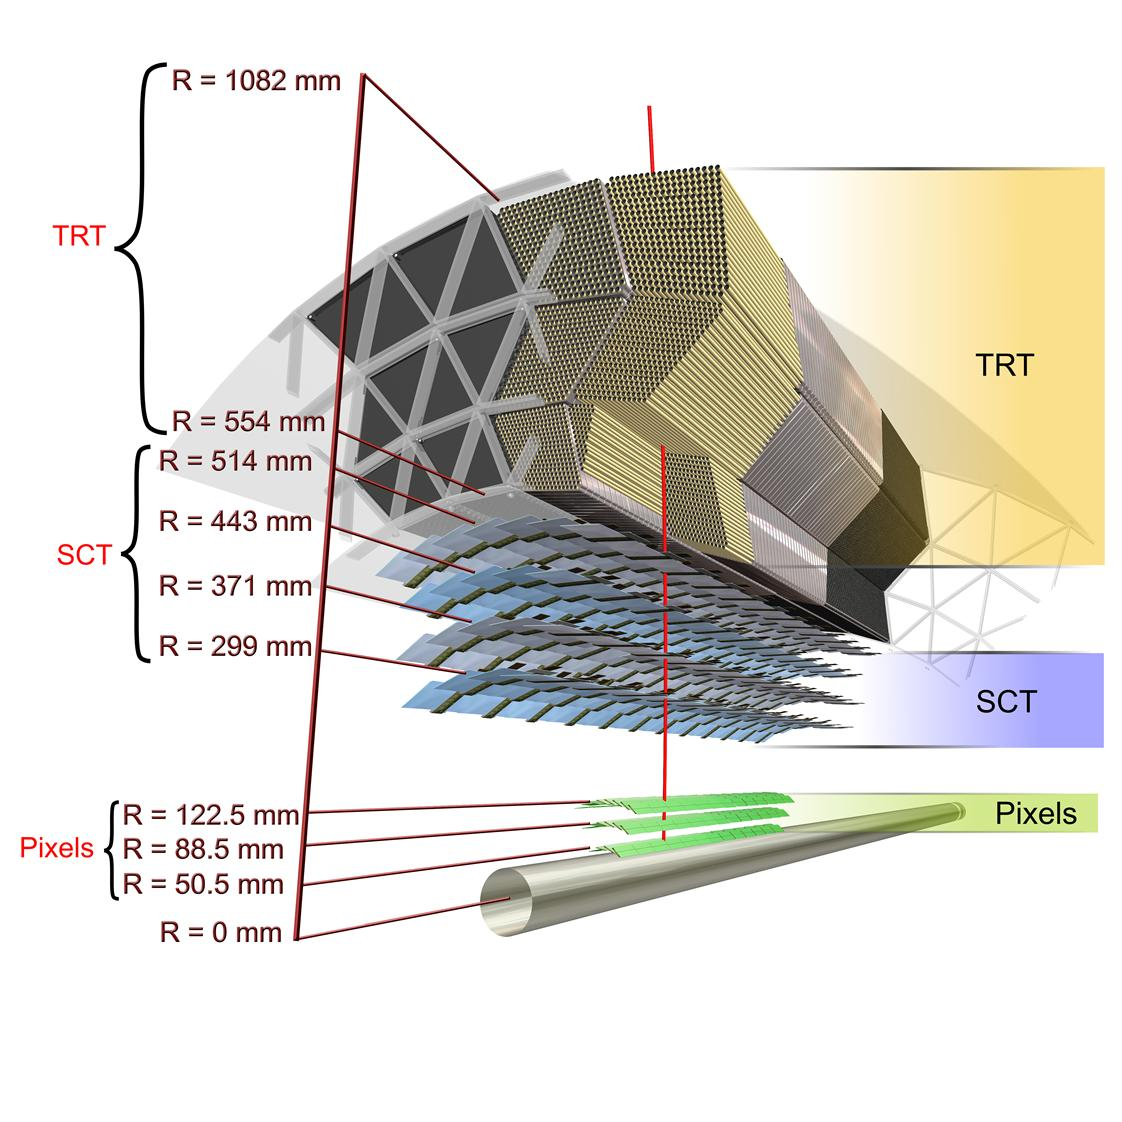
\includegraphics[width=\textwidth, trim=0 2.5cm 0 1cm,
    clip]{atlas/atlas_indet_2}%
    \subcaption{}%
    \label{fig:indet_barrel}
  \end{subfigure}

  \caption[Overview of the ATLAS inner detector.]{Schematic view of the ID
    including the two end-caps (a). A zoomed in view of the barrel region of the
    ID (b). The Insertable B-Layer (IBL), which was introduced into the ATLAS
    detector after Run~1 of the LHC, is not displayed. The IBL is located
    closest to the beampipe at a radius of
    $r = \SI{33.5}{\milli\metre}$~\cite{ATLAS-TDR-19,PIX-2018-001}. The images
    are taken from Ref.~\cite{PERF-2007-01}.}%
  \label{fig:atlas_inner_detector}
\end{figure}

The requirements on the tracking system vary with the distance from the IP.
Closest to the IP, tracking detectors with high-granularity are required for the
reconstruction of primary and secondary vertices that can operate in a
high-radiation environment. At larger distances, the particle flux is
significantly reduced and the requirements on the spatial resolution relaxed.
Therefore, different detector technologies are used to cover the needs of the
tracking system in a cost-effective manner.

% Pixel
The ID sub-system closest to the beampipe are the pixel detectors located at
distances of \SIrange{33.5}{122.5}{\milli\metre} from the beamline in the barrel
region of the ATLAS detector (cf.\ \Cref{fig:atlas_inner_detector}). The pixel
detectors are based on semiconductor technology with an active detector area
that is segmented into a grid of rectangular elements, referred to as
pixels. These pixels have size of \SI{50}{\micro\metre} in the transverse
direction and \SIrange{250}{400}{\micro\metre} along the
beamline~\cite{PERF-2007-01,PIX-2018-001}. A charged particle traversing the
pixel detector ionises the active detector material leading to the deposition of
electric charge in nearby pixels. The charge deposited in individual pixels can
be read out to determine the point where the particle crossed the detector
layer. The pixel detectors are arranged in four layers concentric with the
beamline in the barrel region and three disks per end-cap region. Particles
produced at the IP typically traverse four layers of pixel detectors within the
acceptance of $|\eta| < 2.5$ of the tracking system.

% SCT
The pixel detector is surrounded by the \emph{Semiconductor Tracker} (SCT)
covering radii of \SIrange{299}{514}{\milli\metre} from the beamline in the
barrel region (cf.\ \Cref{fig:atlas_inner_detector}). Similar to the pixel
detector, the SCT is based on semiconductor detector technology, however, the
active detector area is segmented in long but thin strips (microstrips) with a
pitch between strips of about \SI{80}{\micro\metre}~\cite{PERF-2007-01}. A
single microstrip detector layer only provides a position measurement in the
plane perpendicular to the strips. Therefore, SCT modules consist of two layers
of microstrips which are tilted by a small angle to resolve the ambiguity in the
direction parallel to the strips. The SCT is arranged in four layers in the
barrel and nine disks in the end-cap region, yielding at least four measurements
for tracks within the acceptance of the tracking system~\cite{PERF-2007-01}.

% TRT
The \emph{Transition Radiation Tracker} (TRT) is the final layer of the ID
covering radii of \SIrange{554}{1082}{\milli\metre} (cf.\
\Cref{fig:atlas_inner_detector}), however, with reduced acceptance of
$|\eta| < 2.0$ compared to the semiconductor-based trackers. The TRT consists of
about \num{300000} straw-tube chambers, which are gaseous ionisation detectors,
with a diameter of \SI{4}{\milli\metre} arranged in up to 73 layers in the
barrel region and 160 planes in the end-caps~\cite{PERF-2007-01}. The straw-tube
chambers determine the radius at which an ionising particle passed through the
tube, however, no position information parallel to the straw-tubes is obtained.
% The straw-tube chambers consist of gas-filled, electrically conductive tubes
% serving as cathodes with an anode wire passing through the centre of the
% tubes. Charged particles passing through the tubes ionise the gas, the
% resulting electrons/ions being accelerated towards the anode/cathode.
The straw-tubes of the TRT are interleaved with polypropylene fibres (foils) in
the barrel (end-cap) region~\cite{PERF-2007-01}. These fibres/foils provide
interfaces between different dielectric media at which ultrarelativistic
particles can emit transition radiation in the form of
X-rays~\cite{Grupen:2008zz}. At the energies of particles produced at the ATLAS
experiment, the emission of transition radiation is only relevant for electrons
and positrons. The X-rays emitted by electrons/positrons at the interfaces are
absorbed in the xenon-based gas-mixture\footnote{Selected drift tubes affected
  by gas leaks are operated using a cheaper, argon-based gas
  mixture~\cite{IDET-2015-01}.} inside the straw-tubes, leading to measurably
higher ionisation compared to a charged particle passing through the drift
tube. This sensitivity of the TRT to transition radiation is used to identify
electrons and positrons.
% Proportional to the Lorentz factor and thus most relevant for light particles.

\subsection{The Calorimeter System}%
\label{sec:atlas_calorimeters}


The ATLAS calorimeter system, schematically depicted in
\Cref{fig:atlas_calorimeters}, surrounds the ID and is used to perform
destructive measurements of the energy of most charged and neutral particles. Of
the particles predicted by the SM, only muons and neutrinos can traverse the
ATLAS calorimeter system without being absorbed. The calorimeter system covers a
pseudorapidity range of $|\eta| < 4.9$, thus instrumenting almost the full solid
angle surrounding the IP. This is important to prevent detectable particles from
avoiding detection, which consequently allows to determine the sum of transverse
momentum carried away by undetectable particles such as neutrinos or non- or
only weakly-interacting particles from BSM theories, the so-called missing
transverse momentum (\Cref{sec:atlas_met}).

% \todo[inline]{Calorimetry is complementary to charged-particle
% tracking. Energy / momentum resolution and dependency on E / p.}

\begin{figure}[htbp]
  \centering

  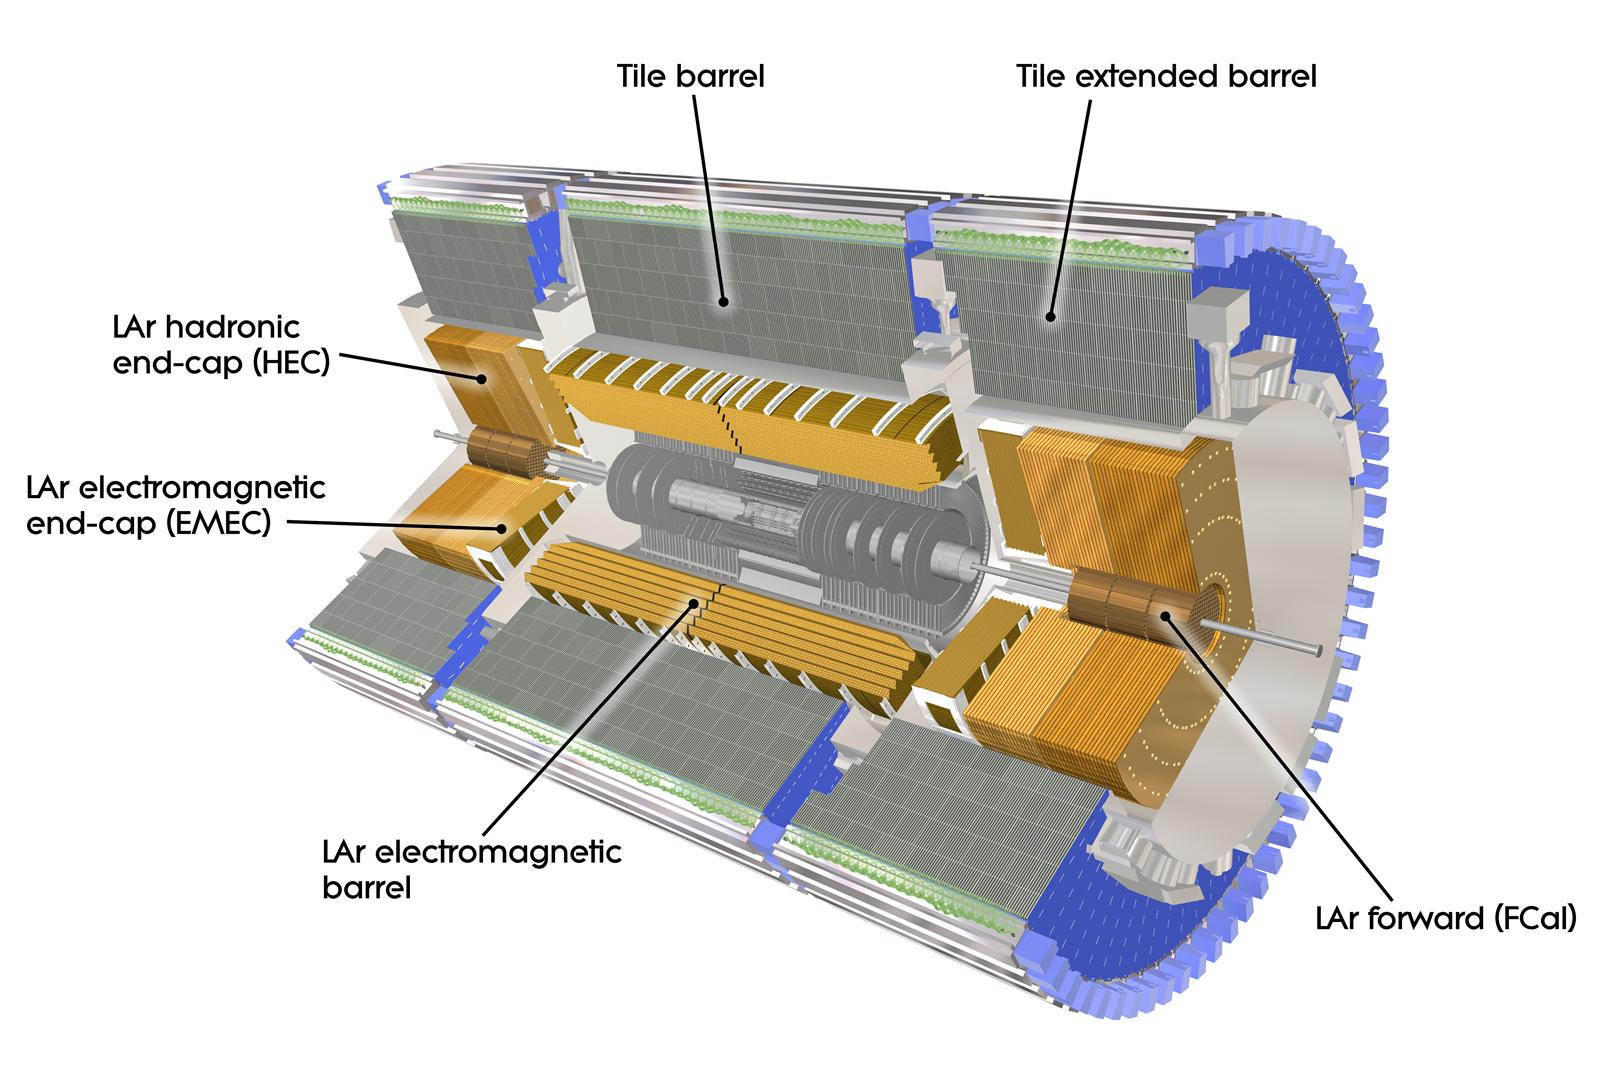
\includegraphics[width=0.65\textwidth]{atlas/atlas_calo}

  \caption[Overview of the ATLAS calorimeter system.]{Overview of the ATLAS
    calorimeter system. The image is taken from Ref.~\cite{PERF-2007-01}.}%
  \label{fig:atlas_calorimeters}
\end{figure}

The ATLAS calorimeter is split into two major parts. The \emph{electromagnetic
  calorimeter}, the innermost part of the calorimeter, is used to measure the
energies of electrons/positrons and photons. It is followed by the
\emph{hadronic calorimeter} which measures the energy of charged and neutral
hadrons that are able to pass through the electromagnetic calorimeter. This
design is governed by the interactions of particles with matter at the energy
scales relevant for the ATLAS experiment. Highly energetic electrons/positrons
and photons interact with the calorimeter material by emitting Bremsstrahlung
and converting into electron--positron pairs, respectively. This process occurs
repeatedly, producing a cascade of electrons, positrons, and photons, until the
energy of the constituent particles is sufficiently small to be absorbed in the
material. These cascades, referred to as \emph{electromagnetic showers}, are
homogeneous and compact with high energy density. The dimensions of the
electromagnetic calorimeters are chosen such that they fully contain
electromagnetic showers originating from promptly produced electrons/positrons
and photons. The interactions of hadrons with the calorimeter material are
driven by nuclear interactions which also result in cascades of secondary
particles. A variety of processes are relevant for the evolution of these
so-called \emph{hadronic showers}, for example: inelastic scattering of hadrons
at nuclei, spallation, fission, or neutron
capture~\cite{Kolanoski:2016gyf}. Moreover, electromagnetic showers are an
important sub-component of hadronic showers which, for example, originate from
photons produced in $\pi^0$ decays. The length scales of hadronic showers are
larger, both laterally and longitudinally, than the ones of electromagnetic
showers.
% Moreover, hadronic showers show localised fluctuations distinguishing them from
% the homogenous electromagnetic showers.
This is reflected in the design of the ATLAS calorimeter system with the
hadronic calorimeter having almost four times the radial thickness of the
electromagnetic calorimeter~\cite{ATLAS-TDR-02,ATLAS-TDR-03}.

The electromagnetic and hadronic calorimeters are sampling calorimeters, i.e.\
they consist of alternating layers of absorber material for shower development
and active detector layers that sample the shower as it develops. Depending on
the part of the calorimeter, the active detector layers are either ionisation
chambers filled with liquid argon (LAr) or plastic scintillator tiles connected
to photomultiplier tubes.


\subsubsection{Electromagnetic Calorimeters}

The electromagnetic calorimeter of the ATLAS detector (cf.\
\Cref{fig:atlas_calorimeters}) is divided into a barrel ($|\eta| < 1.475$),
end-cap ($1.375 < |\eta| < 3.2$), and forward ($3.1 < |\eta| < 4.9$)
region~\cite{PERF-2007-01}. The electromagnetic calorimeters in the barrel and
end-cap region consist of lead absorbers with LAr-filled gaps that are
instrumented with electrodes to form ionisation chambers. The calorimeter is
segmented both laterally and longitudinally, with varying granularity, to
provide information on the location and shape of showers in the calorimeter. The
forward electromagnetic calorimeter uses copper absorbers and a single
longitudinal layer instead.
% Additionally, the region of $|\eta| < 1.8$ in front
% of the calorimeter is instrumented with a so-called pre-sampler, which is a
% thin layer of LAr-based calorimeter used to


\subsubsection{Hadronic Calorimeters}

The hadronic calorimeter (cf.\ \Cref{fig:atlas_calorimeters}) is divided into a
barrel ($|\eta| < 1.0$), extended barrel ($0.8 < |\eta| < 1.7$), end-cap
($1.5 < |\eta| < 3.2$), and forward ($3.1 < |\eta| < 4.9$)
region~\cite{PERF-2007-01}.  The barrel and extended barrel calorimeter consists
of alternating steel plates and plastic scintillator tiles. The scintillators
are connected via optical fibres to photomultiplier tubes for readout. The
hadronic end-cap calorimeter (HEC) and forward calorimeter consist of LAr-filled
ionisation chambers with copper and tungsten absorbers, respectively. The
hadronic calorimeter is also segmented laterally and longitudinally, although
with reduced granularity compared to the electromagnetic calorimeter.


\subsection{The Muon Spectrometer}%
\label{sec:atlas_ms}

The MS, shown in \Cref{fig:atlas_muon_system}, is the outermost and largest part
of the ATLAS detector. It is a tracking detector providing independent momentum
measurements of muons that pass the calorimeters. The active detector elements
of the MS are based on gaseous ionisation detectors for cost-effective
instrumentation of large areas. The MS provides a coverage of $|\eta| < 2.7$ for
precision tracking and $|\eta| < 2.4$ for triggering on muons.

\begin{figure}[htbp]
  \centering

  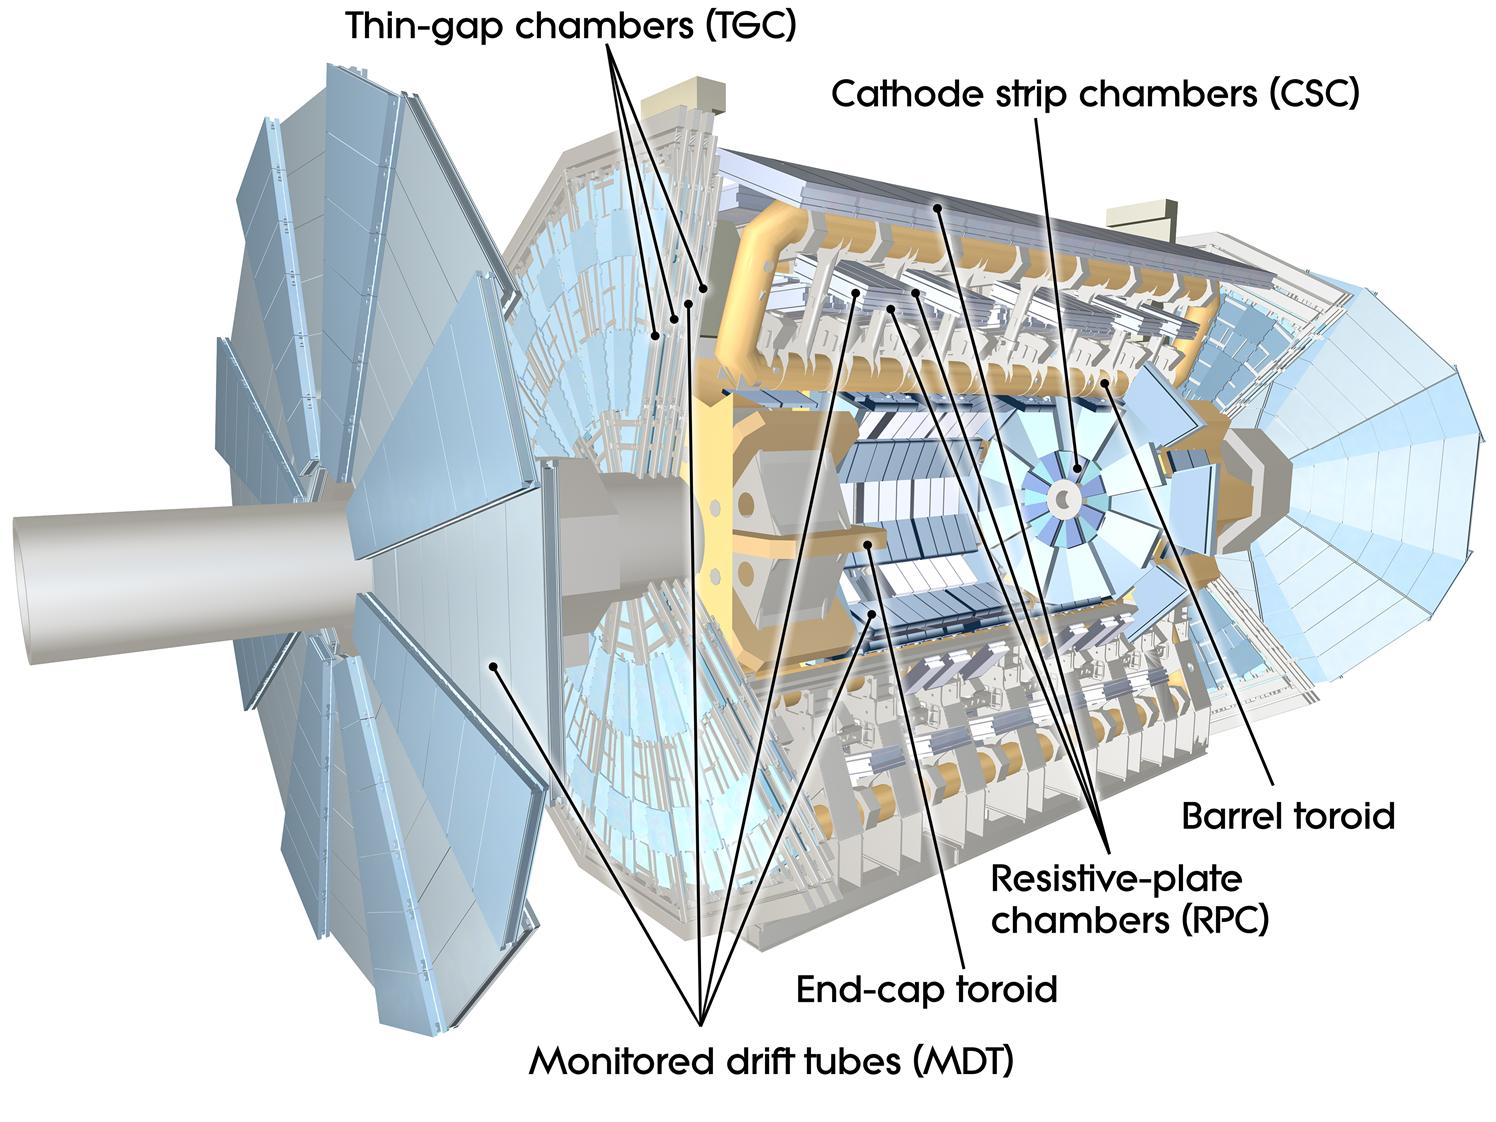
\includegraphics[width=0.56\textwidth]{atlas/atlas_muon}

  \caption[Overview of the ATLAS muon spectrometer.]{Overview of the ATLAS muon
    spectrometer. The image is taken from Ref.~\cite{PERF-2007-01}.}%
  \label{fig:atlas_muon_system}
\end{figure}

The ATLAS detector uses multiple layers monitored drift tube
chambers\footnote{Deformations of the muon chambers are actively monitored using
  an optical alignment system built into the frame of the chambers.} (MDTs) for
precision tracking in $|\eta| < 2.7$. To cope with the large rate of incident
particles in the forward region, the innermost layer in $2.0 < |\eta| < 2.7$ is
replaced by cathode strip chambers (CSCs). The MS is complemented with resistive
plate chambers (RPCs) and thin gap chambers (TGCs) in the barrel
($|\eta| < 1.05$) and end-cap ($1.05 < |\eta| < 2.7$) region, respectively,
providing the necessary timing information to identify the bunch crossing a muon
originates from. The MS is arranged, as depicted
in~\Cref{fig:atlas_muon_system}, in three cylindrical layers surrounding the LHC
beamline in the barrel region. A gap in the instrumentation of the MS is left at
$\eta = 0$ for access to the inner parts of the detector for servicing. The
end-cap region is instrumented by muon chambers in the form of three wheels
perpendicular to the beampipe. A \emph{small wheel} is located in front of the
end-cap toroid, and two \emph{big wheels} are located behind the end-cap
toroid. Every layer/wheel consists of multiple tracking planes.


\subsection{The ATLAS Trigger System}%
\label{sec:atlas_trigger}

With a peak bunch crossing rate of \SI{40}{\mega\hertz} and an expected number
of inelastic \pp~collisions in a single bunch crossing of around \num{30} (cf.\
\Cref{fig:lumi_and_pu}), it is not possible to record every collision event due
to limitations in the detector read-out and data storage. However, most
collision events are not of particular interest to the physics programme of the
ATLAS experiment. For example, events containing a weak vector boson decaying
into leptons are expected to occur about once every $10^6$ inelastic
\pp~collisions at $\sqrt{s} = \SI{13}{\TeV}$~\cite{STDM-2015-03}. Other
processes, such as the production of Higgs bosons, are multiple orders of
magnitude less frequent than the production of $Z$ and $W$ bosons.

The task of the ATLAS trigger system~\cite{TRIG-2019-04} is to reduce the rate
at which events are recorded by performing an event pre-selection already during
data-taking (\emph{online}). This is achieved by monitoring the ATLAS detector
for signatures of rare physics processes, for example indicated by the presence
of charged leptons with large transverse momenta. A multitude of different event
selections, usually referred to as \emph{triggers}, are implemented in the ATLAS
trigger system to target the signatures of different physics processes. The
implementation of these triggers are heavily constrained due to the limited
detector read-out and strict latency and bandwidth constraints. Due to the
increasing instantaneous luminosity during Run~2 of the LHC, the triggers
employed by the ATLAS experiment had to evolve to meet the bandwidth
requirements. Therefore, the exact selections of triggers targeting particular
signatures changed as Run~2 progressed. During Run~2, the ATLAS trigger system
reduced the rate of selected events to about
\SI{1.2}{\kilo\hertz}~\cite{TRIG-2019-04} which could be recorded for
(\emph{offline}) analysis.

The ATLAS trigger system consists of two stages. The first stage, called the
Level-1 (L1) trigger, implements the event selection in hardware using custom
electronic circuits. At the L1 trigger, only calorimeter and MS information with
reduced granularity can be used for selection. The rate of accepted events is
reduced to \SI{100}{\kilo\hertz}~\cite{TRIG-2019-04} by the L1 trigger. If an
event is accepted, all sub-detectors of the ATLAS experiment are read-out and
the data are sent to the second stage of the trigger system, the so-called
High-Level Trigger (HLT). The HLT is software-based and runs reconstruction
algorithms similar to those applied during offline event reconstruction.  Event
selections at the HLT are staged into \emph{chains} of algorithms with
increasing computational/time complexity. A given HLT chain is only applied to
events selected by particular L1 triggers, usually referred to as the L1 seed of
the chain. The selections applied by the HLT reduces the mean rate of accepted
events to the target of \SI{1.2}{\kilo\hertz}~\cite{TRIG-2019-04}.


%%% Local Variables:
%%% mode: latex
%%% TeX-master: "../../phd_thesis"
%%% End:
